\documentclass[conference]{IEEEtran}
\IEEEoverridecommandlockouts
% The preceding line is only needed to identify funding in the first footnote. If that is unneeded, please comment it out.
\usepackage{cite}
\usepackage{amsmath,amssymb,amsfonts}
\usepackage{algorithmic}
\usepackage{graphicx}
\usepackage{textcomp}
\usepackage{xcolor}
\usepackage{tikz}
\usepackage{pgfplots}
\usepackage{tcolorbox}
\usepackage{colortbl}
\usepackage{dirtree}
\usepackage{longtable}
\usepackage{booktabs}
\usepackage{xeCJK}
\usepackage{float}

\def\BibTeX{{\rm B\kern-.05em{\sc i\kern-.025em b}\kern-.08em
    T\kern-.1667em\lower.7ex\hbox{E}\kern-.125emX}}

\begin{document}

\setCJKfamilyfont{songti}{STZhongsong}\newcommand{\STSong}{\CJKfamily{STSong}} % Move this line inside the document environment

论文\cite{zhao2021merge}介绍的SMerge(即NN-Merge)是一种基于NNDescent的合并KNN图的方法。通过复现论文中给出的算法,利用sift-10k数据集,将数据集一分为二分别使用NNDescent建立近似最近邻图,使用SMerge进行了测试合并,测量各部分耗时。

\begin{figure}[H]
    \begin{center}
        \includegraphics[width=1.0\linewidth]{image.png}
        \caption{SMerge算法各部分耗时}
        \label{fig1}
    \end{center}
\end{figure}

使用的数据集较小,因为主要的耗时都集中在NNDescent,图\ref{fig1}可以直观体现主要耗时的部分。在sift-1m数据集下,NNDescent的耗时占比超过了99\%。
因此,NNDescent的速度决定了图合并的速度。
论文\cite{ono2023relative}中提供的RNN-Descent方法可以很大程度上改进这一点。通过复现RNN-Descent,可以发现RNN-Descent能够有效提高图建立的速度。
尝试改进S-Merge,将原有的NNDescent实现替换为RNN-Descent形成RNN-Merge。测试中,利用sift-1m数据集,将数据集一分为二分别使用NNDescent建立近似最近邻图,使用RNN-Merge进行合并。

\begin{figure}[H]
    \centering
    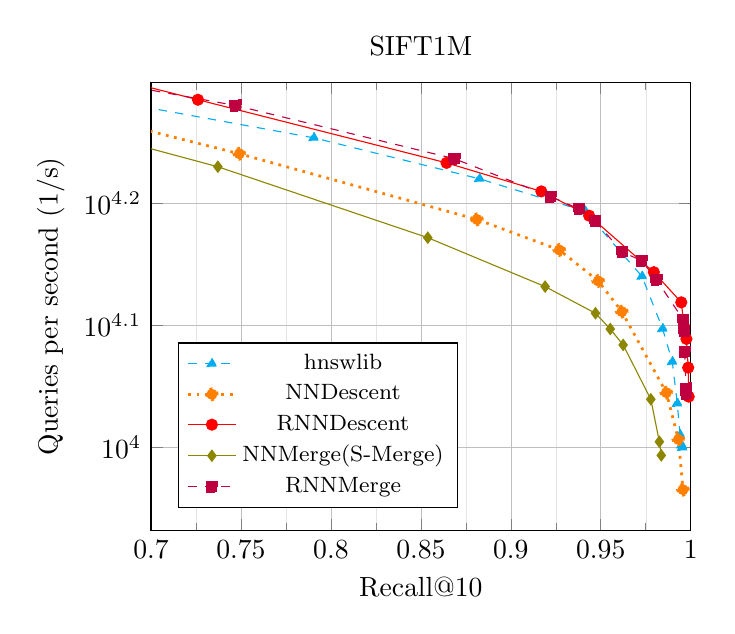
\begin{tikzpicture}
        \begin{axis}[
            xlabel={ Recall@10 },
            ylabel={ Queries per second (1/s) },
            ymode = log,
            xmin=0.7,
            xmax=1,
            ymax={10^4.3},
            % ymin={10^4},
            xtick={0.7, 0.75, 0.8, 0.85, 0.9, 0.95, 1},
            yticklabel style={/pgf/number format/fixed,
                              /pgf/number format/precision=3},
            legend style={font=\footnotesize, at={(0.05,0.05)}, anchor=south west},
            cycle list name = black white,
            grid=both,
            major grid style={line width=.2pt,draw=gray!50}, 
            minor grid style={line width=.1pt,draw=gray!20}, 
            minor tick num=1,
            title={SIFT1M}
            ]

            \addplot[  mark=triangle*, color=cyan, dashed] coordinates {
                (0.61348, 20032.9)
                (0.79049, 17958.7)
                (0.88257, 16620.27)
                (0.94136, 15628.6)
                (0.97293, 13820.83)
                (0.98439, 12517.6)
                (0.98978, 11760.70)
                (0.99257, 10870.64)
                (0.99405, 10246.2)
                (0.99496, 10047.7)
                (0.99545, 10002.9)
            };
            \addlegendentry{hnswlib};

            \addplot[dotted,line width=1pt, mark=*, color=orange]  coordinates{
                (0.61429, 19556.8)
                (0.74911, 17425.1)
                (0.88119, 15391.5)
                (0.92698, 14528.6)
                (0.94861, 13701.8)
                (0.96176, 12931)
                (0.98647, 11095.2)
                (0.99318, 10156.7)
                (0.99573, 9236.68)
            };
            \addlegendentry{NNDescent};

            \addplot[mark=*, color=red] coordinates{
                (0.61429, 21256.8)
                (0.72608, 19299)
                (0.86428, 17127.8)
                (0.91698, 16228.6)
                (0.94353, 15501.8)
                (0.97951, 13931)
                (0.99477, 13159.7)
                (0.99639, 12567.8)
                (0.99762, 12281.1)
                (0.99862, 11632.6)
                (0.99889, 11012.4)
            };
            \addlegendentry{RNNDescent}

            \addplot[ mark=diamond*, color=olive] coordinates{
                (0.61225, 19059.9)
                (0.73715, 17001.8)
                (0.85384, 14868.9)
                (0.91908, 13556.7)
                (0.94708, 12890.1)
                (0.95528, 12513.4)
                (0.96245, 12142)
                (0.97785, 10956.5)
                (0.98259, 10112.9)
                (0.98366, 9855.98)
            };
            \addlegendentry{NNMerge(S-Merge)}

            \addplot[mark=square*, color=purple, dashed]  coordinates{
                (0.61879, 20658.7)
                (0.74692, 19091.3)
                (0.86865, 17262.5)
                (0.92223, 16067.6)
                (0.93795, 15700.6)
                (0.94685, 15345.6)
                (0.96195, 14473.7)
                (0.97284, 14235.9)
                (0.98097, 13733.4)
                (0.99594, 12733.2)
                (0.99647, 12465.9)
                (0.99671, 11986)
                (0.99744, 11181.6)
                (0.99752, 11076.2)
            };
            \addlegendentry{RNNMerge}

            \end{axis}
    \end{tikzpicture}
    \caption{ Recall-Queries per second (1/s) tradeoff - up and to the right is better}
    \label{fig2}
\end{figure}

\begin{figure}[H]
    \centering
    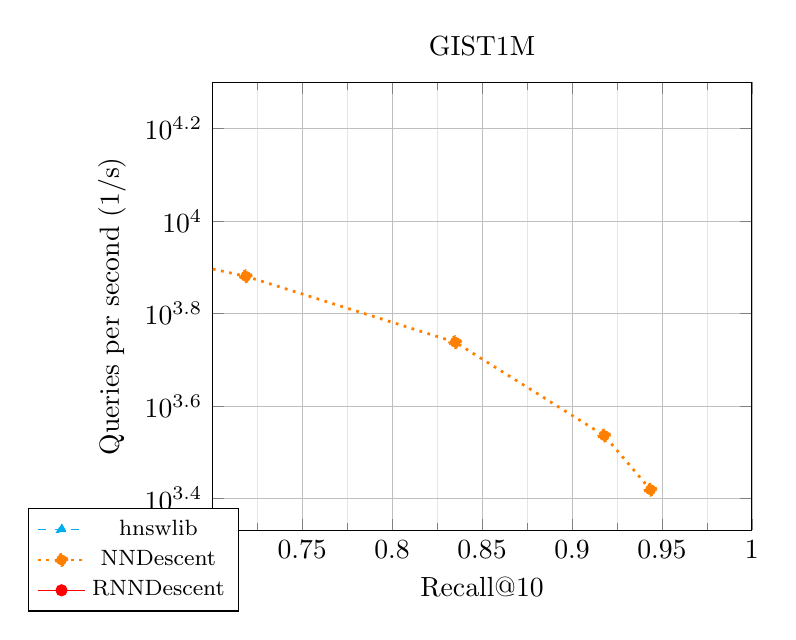
\begin{tikzpicture}
        \begin{axis}[
            xlabel={ Recall@10 },
            ylabel={ Queries per second (1/s) },
            ymode = log,
            xmin=0.7,
            xmax=1,
            ymax={10^4.3},
            xtick={0.7, 0.75, 0.8, 0.85, 0.9, 0.95, 1},
            yticklabel style={/pgf/number format/fixed,
                              /pgf/number format/precision=3},
            legend style={font=\footnotesize, at={(0.05,0.05)}, anchor=north east},
            cycle list name = black white,
            grid=both,
            major grid style={line width=.2pt,draw=gray!50}, 
            minor grid style={line width=.1pt,draw=gray!20}, 
            minor tick num=1,
            title={GIST1M}
            ]

            \addplot[  mark=triangle*, color=cyan, dashed] coordinates {
                (0.6654, 12646.5)
                

            };
            \addlegendentry{hnswlib};

            \addplot[dotted,line width=1pt, mark=*, color=orange]  coordinates{
                (0.6778, 8224.43)
                (0.7187, 7597.8)
                (0.8351, 5472.96)
                (0.918, 3439.87)
                (0.9437, 2626.79)
            };
            \addlegendentry{NNDescent};

            \addplot[mark=*, color=red] coordinates{
                (0.6648, 9384.04)
                
            };
            \addlegendentry{RNNDescent}

            \addplot[ mark=diamond*, color=olive] coordinates{
                
            };
            \addlegendentry{NNMerge(S-Merge)}

            \addplot[mark=square*, color=purple, dashed]  coordinates{
                
            };
            \addlegendentry{RNNMerge}

            \end{axis}
    \end{tikzpicture}
    \caption{ Recall-Queries per second (1/s) tradeoff - up and to the right is better}
    \label{fig3}
\end{figure}

\begin{figure}[H]
    \centering
    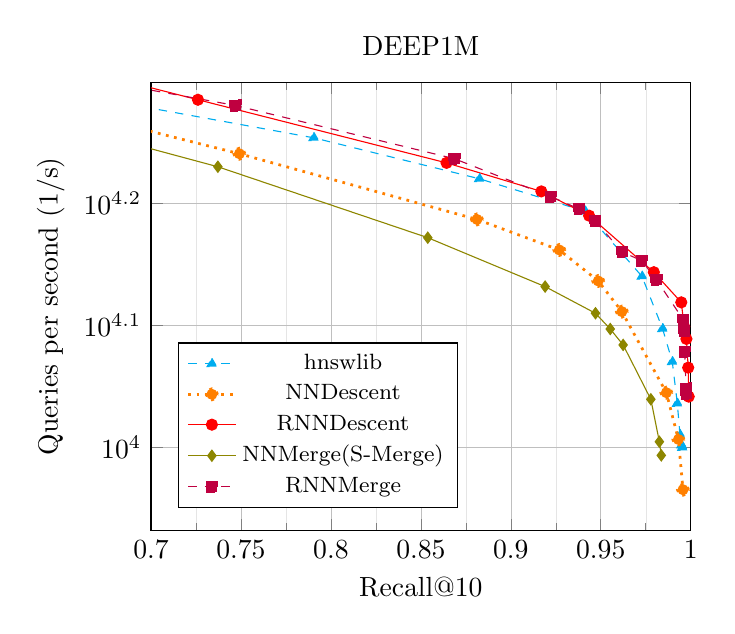
\begin{tikzpicture}
        \begin{axis}[
            xlabel={ Recall@10 },
            ylabel={ Queries per second (1/s) },
            ymode = log,
            xmin=0.7,
            xmax=1,
            ymax={10^4.3},
            % ymin={10^4},
            xtick={0.7, 0.75, 0.8, 0.85, 0.9, 0.95, 1},
            yticklabel style={/pgf/number format/fixed,
                              /pgf/number format/precision=3},
            legend style={font=\footnotesize, at={(0.05,0.05)}, anchor=south west},
            cycle list name = black white,
            grid=both,
            major grid style={line width=.2pt,draw=gray!50}, 
            minor grid style={line width=.1pt,draw=gray!20}, 
            minor tick num=1,
            title={DEEP1M}
            ]

            \addplot[  mark=triangle*, color=cyan, dashed] coordinates {
                (0.61348, 20032.9)
                (0.79049, 17958.7)
                (0.88257, 16620.27)
                (0.94136, 15628.6)
                (0.97293, 13820.83)
                (0.98439, 12517.6)
                (0.98978, 11760.70)
                (0.99257, 10870.64)
                (0.99405, 10246.2)
                (0.99496, 10047.7)
                (0.99545, 10002.9)
            };
            \addlegendentry{hnswlib};

            \addplot[dotted,line width=1pt, mark=*, color=orange]  coordinates{
                (0.61429, 19556.8)
                (0.74911, 17425.1)
                (0.88119, 15391.5)
                (0.92698, 14528.6)
                (0.94861, 13701.8)
                (0.96176, 12931)
                (0.98647, 11095.2)
                (0.99318, 10156.7)
                (0.99573, 9236.68)
            };
            \addlegendentry{NNDescent};

            \addplot[mark=*, color=red] coordinates{
                (0.61429, 21256.8)
                (0.72608, 19299)
                (0.86428, 17127.8)
                (0.91698, 16228.6)
                (0.94353, 15501.8)
                (0.97951, 13931)
                (0.99477, 13159.7)
                (0.99639, 12567.8)
                (0.99762, 12281.1)
                (0.99862, 11632.6)
                (0.99889, 11012.4)
            };
            \addlegendentry{RNNDescent}

            \addplot[ mark=diamond*, color=olive] coordinates{
                (0.61225, 19059.9)
                (0.73715, 17001.8)
                (0.85384, 14868.9)
                (0.91908, 13556.7)
                (0.94708, 12890.1)
                (0.95528, 12513.4)
                (0.96245, 12142)
                (0.97785, 10956.5)
                (0.98259, 10112.9)
                (0.98366, 9855.98)
            };
            \addlegendentry{NNMerge(S-Merge)}

            \addplot[mark=square*, color=purple, dashed]  coordinates{
                (0.61879, 20658.7)
                (0.74692, 19091.3)
                (0.86865, 17262.5)
                (0.92223, 16067.6)
                (0.93795, 15700.6)
                (0.94685, 15345.6)
                (0.96195, 14473.7)
                (0.97284, 14235.9)
                (0.98097, 13733.4)
                (0.99594, 12733.2)
                (0.99647, 12465.9)
                (0.99671, 11986)
                (0.99744, 11181.6)
                (0.99752, 11076.2)
            };
            \addlegendentry{RNNMerge}

            \end{axis}
    \end{tikzpicture}
    \caption{ Recall-Queries per second (1/s) tradeoff - up and to the right is better}
    \label{fig4}
\end{figure}


\begin{figure}[H]
    \centering
    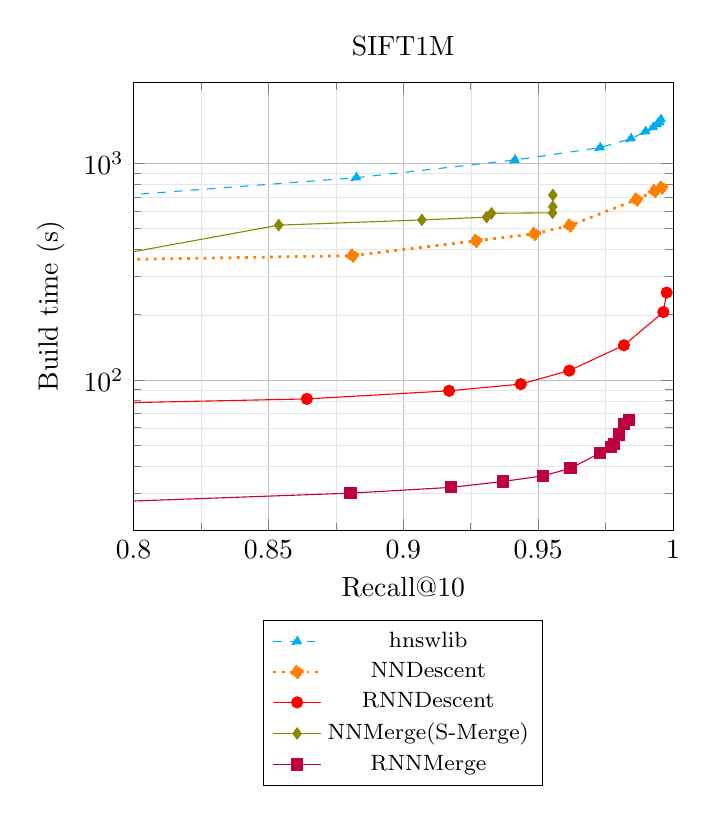
\begin{tikzpicture}
        \begin{axis}[
            xlabel={ Recall@10 },
            ylabel={ Build time (s) },
            ymode = log,
            yticklabel style={/pgf/number format/fixed,
                              /pgf/number format/precision=3},
            xmin=0.80,
            xmax=1,
            legend style={font=\footnotesize, at={(0.5,-0.2)}, anchor=north},
            cycle list name = black white,
            grid=both,
            major grid style={line width=.2pt,draw=gray!50}, 
            minor grid style={line width=.1pt,draw=gray!20}, 
            minor tick num=1,
            title={SIFT1M}
            ]
            \addplot[mark=triangle*, color=cyan, dashed] coordinates {
                (0.79049, 703.37)
                (0.88257, 859.397)
                (0.94136, 1037.61)
                (0.97293, 1182.7)
                (0.98439, 1301.27)
                (0.98978, 1403.83)
                (0.99257, 1466.91)
                (0.99405, 1516.61)
                (0.99496, 1544.56)
                (0.99545, 1595.92)
            };
            \addlegendentry{hnswlib};
            \addplot[dotted,line width=1pt, mark=*, color=orange] coordinates{
                (0.74911, 351.521)
                (0.88119, 374.881)
                (0.92698, 438.879)
                (0.94861, 472.64)
                (0.96176, 516.336)
                (0.98647, 680.832)
                (0.99318, 745.693)
                (0.99573, 773.159)
            };
            \addlegendentry{NNDescent}

            \addplot[mark=*, color=red] coordinates{
                (0.72608, 75.0176)
                (0.86428, 81.5669)
                (0.91698, 88.9337)
                (0.94353, 95.4841)
                (0.96153, 110.276)
                (0.98177, 144.389)
                (0.99639, 205.514)
                (0.99762, 253.026)
            };
            \addlegendentry{RNNDescent}

            \addplot[mark=diamond*, color=olive] coordinates{
                (0.73715, 281.019)
                (0.85384, 518.534)
                (0.90689, 548.298)
                (0.93089, 564.782)
                (0.93273, 588.235)
                (0.95533, 591.532)
                (0.95541, 631.332)
                (0.95545, 714.818)
            };
            \addlegendentry{NNMerge(S-Merge)}

            \addplot[mark=square*, color=purple] coordinates{
                (0.74692, 26.0325)
                (0.88046, 29.9219)
                (0.91773, 31.8162)
                (0.93697, 33.8883)
                (0.95175, 35.9472)
                (0.96195, 38.97)
                (0.97284, 45.8013)
                (0.97714, 48.9931)
                (0.97813, 50.4851)
                (0.97986, 55.8476)
                (0.98169, 62.3913)
                (0.98365, 65.2466)
            };
            \addlegendentry{RNNMerge}
            
            
            \end{axis}
    \end{tikzpicture}
    \caption{ Recall-Build time (s) tradeoff - down and to the right is better}
    \label{fig5}
\end{figure}


\begin{figure}[H]
    \centering
    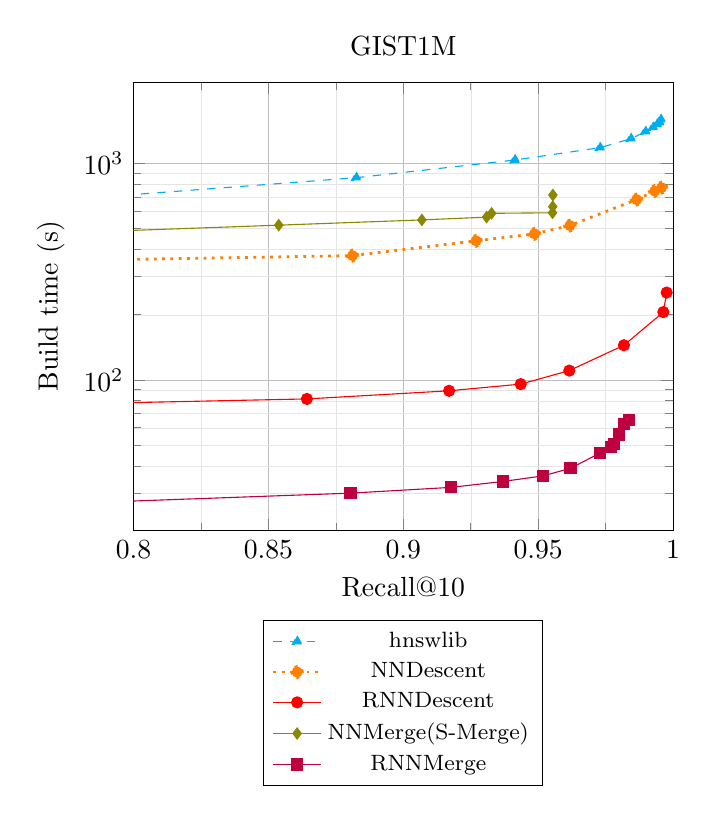
\begin{tikzpicture}
        \begin{axis}[
            xlabel={ Recall@10 },
            ylabel={ Build time (s) },
            ymode = log,
            yticklabel style={/pgf/number format/fixed,
                              /pgf/number format/precision=3},
            xmin=0.80,
            xmax=1,
            legend style={font=\footnotesize, at={(0.5,-0.2)}, anchor=north},
            cycle list name = black white,
            grid=both,
            major grid style={line width=.2pt,draw=gray!50}, 
            minor grid style={line width=.1pt,draw=gray!20}, 
            minor tick num=1,
            title={GIST1M}
            ]
            \addplot[mark=triangle*, color=cyan, dashed] coordinates {
                (0.79049, 703.37)
                (0.88257, 859.397)
                (0.94136, 1037.61)
                (0.97293, 1182.7)
                (0.98439, 1301.27)
                (0.98978, 1403.83)
                (0.99257, 1466.91)
                (0.99405, 1516.61)
                (0.99496, 1544.56)
                (0.99545, 1595.92)
            };
            \addlegendentry{hnswlib};
            \addplot[dotted,line width=1pt, mark=*, color=orange] coordinates{
                (0.74911, 351.521)
                (0.88119, 374.881)
                (0.92698, 438.879)
                (0.94861, 472.64)
                (0.96176, 516.336)
                (0.98647, 680.832)
                (0.99318, 745.693)
                (0.99573, 773.159)
            };
            \addlegendentry{NNDescent}

            \addplot[mark=*, color=red] coordinates{
                (0.72608, 75.0176)
                (0.86428, 81.5669)
                (0.91698, 88.9337)
                (0.94353, 95.4841)
                (0.96153, 110.276)
                (0.98177, 144.389)
                (0.99639, 205.514)
                (0.99762, 253.026)
            };
            \addlegendentry{RNNDescent}

            \addplot[mark=diamond*, color=olive] coordinates{
                (0.73715, 459.924)
                (0.85384, 518.534)
                (0.90689, 548.298)
                (0.93089, 564.782)
                (0.93273, 588.235)
                (0.95533, 591.532)
                (0.95541, 631.332)
                (0.95545, 714.818)
            };
            \addlegendentry{NNMerge(S-Merge)}

            \addplot[mark=square*, color=purple] coordinates{
                (0.74692, 26.0325)
                (0.88046, 29.9219)
                (0.91773, 31.8162)
                (0.93697, 33.8883)
                (0.95175, 35.9472)
                (0.96195, 38.97)
                (0.97284, 45.8013)
                (0.97714, 48.9931)
                (0.97813, 50.4851)
                (0.97986, 55.8476)
                (0.98169, 62.3913)
                (0.98365, 65.2466)
            };
            \addlegendentry{RNNMerge}
            
            
            \end{axis}
    \end{tikzpicture}
    \caption{ Recall-Build time (s) tradeoff - down and to the right is better}
    \label{fig6}
\end{figure}


\begin{figure}[H]
    \centering
    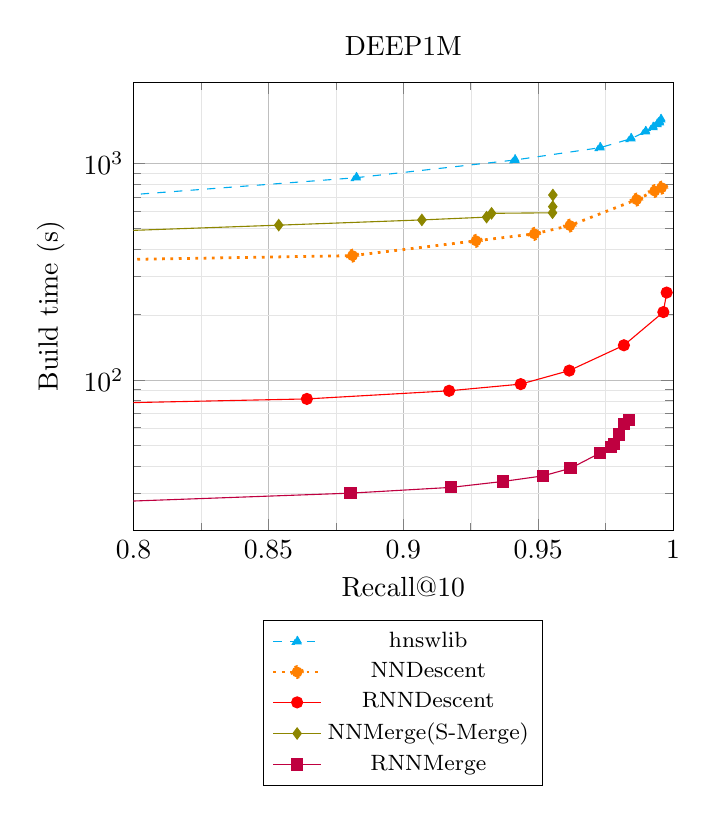
\begin{tikzpicture}
        \begin{axis}[
            xlabel={ Recall@10 },
            ylabel={ Build time (s) },
            ymode = log,
            yticklabel style={/pgf/number format/fixed,
                              /pgf/number format/precision=3},
            xmin=0.80,
            xmax=1,
            legend style={font=\footnotesize, at={(0.5,-0.2)}, anchor=north},
            cycle list name = black white,
            grid=both,
            major grid style={line width=.2pt,draw=gray!50}, 
            minor grid style={line width=.1pt,draw=gray!20}, 
            minor tick num=1,
            title={DEEP1M}
            ]
            \addplot[mark=triangle*, color=cyan, dashed] coordinates {
                (0.79049, 703.37)
                (0.88257, 859.397)
                (0.94136, 1037.61)
                (0.97293, 1182.7)
                (0.98439, 1301.27)
                (0.98978, 1403.83)
                (0.99257, 1466.91)
                (0.99405, 1516.61)
                (0.99496, 1544.56)
                (0.99545, 1595.92)
            };
            \addlegendentry{hnswlib};
            \addplot[dotted,line width=1pt, mark=*, color=orange] coordinates{
                (0.74911, 351.521)
                (0.88119, 374.881)
                (0.92698, 438.879)
                (0.94861, 472.64)
                (0.96176, 516.336)
                (0.98647, 680.832)
                (0.99318, 745.693)
                (0.99573, 773.159)
            };
            \addlegendentry{NNDescent}

            \addplot[mark=*, color=red] coordinates{
                (0.72608, 75.0176)
                (0.86428, 81.5669)
                (0.91698, 88.9337)
                (0.94353, 95.4841)
                (0.96153, 110.276)
                (0.98177, 144.389)
                (0.99639, 205.514)
                (0.99762, 253.026)
            };
            \addlegendentry{RNNDescent}

            \addplot[mark=diamond*, color=olive] coordinates{
                (0.73715, 459.924)
                (0.85384, 518.534)
                (0.90689, 548.298)
                (0.93089, 564.782)
                (0.93273, 588.235)
                (0.95533, 591.532)
                (0.95541, 631.332)
                (0.95545, 714.818)
            };
            \addlegendentry{NNMerge(S-Merge)}

            \addplot[mark=square*, color=purple] coordinates{
                (0.74692, 26.0325)
                (0.88046, 29.9219)
                (0.91773, 31.8162)
                (0.93697, 33.8883)
                (0.95175, 35.9472)
                (0.96195, 38.97)
                (0.97284, 45.8013)
                (0.97714, 48.9931)
                (0.97813, 50.4851)
                (0.97986, 55.8476)
                (0.98169, 62.3913)
                (0.98365, 65.2466)
            };
            \addlegendentry{RNNMerge}
            
            
            \end{axis}
    \end{tikzpicture}
    \caption{ Recall-Build time (s) tradeoff - down and to the right is better}
    \label{fig7}
\end{figure}

图\ref{fig2}和图\ref{fig3}中,NN-Merge的耗时相比NN-Descent直接建立索引要快一些;RNNDescent建立索引的速度很快;在RNNDescent的基础上,RNN-Merge大幅降低了耗时。图索引建立都是基于单线程的。

论文\cite{zhao2021merge}中提供的方法,首先将图中每个点邻居表分成两部分,前半部分$G_u$,后半部分$G_v$,前半部分保留,后半部分随机采样另一个图中的点。即分别给两个图中的点随机选取另一个图中的样本,合并后通过NNDescent来迭代更新图。然而,建图耗时主要集中在更新迭代的过程中,如果可以尽量减少迭代次数,可以大幅提高效率。

参考论文\cite{malkov2018efficient}提供的建图方法,在添加样本时,采用搜索最近邻的方式搜索出每个点在另一个图中可能的邻居,并作为样本添加到该点的候选邻居中。随后再利用RNNDescent迭代更新图,效果预计会更好。

然而,相比于随机采样,为每个点搜索邻居是耗时的,我们假设使用参数beta来控制为每个点搜索邻居的数量。当$beta=0$时,不搜索邻居,直接随机采样;当$beta=1$时,将搜索邻居并填充;当$0<beta<1$时,搜索邻居并填充的数量为$beta*\lvert G_v \rvert$。

图\ref{fig4}展示了不同beta值下的Recall和建图耗时的关系。目前来看,可能还是完全采用搜索效果会更好,此时耗时最短。

总体来讲,利用现有的方法进行knngraph合并的效果相对显著,如sift1m数据集在单线程下在40s即可达到接近1的recall。

\begin{figure}
    \centering
    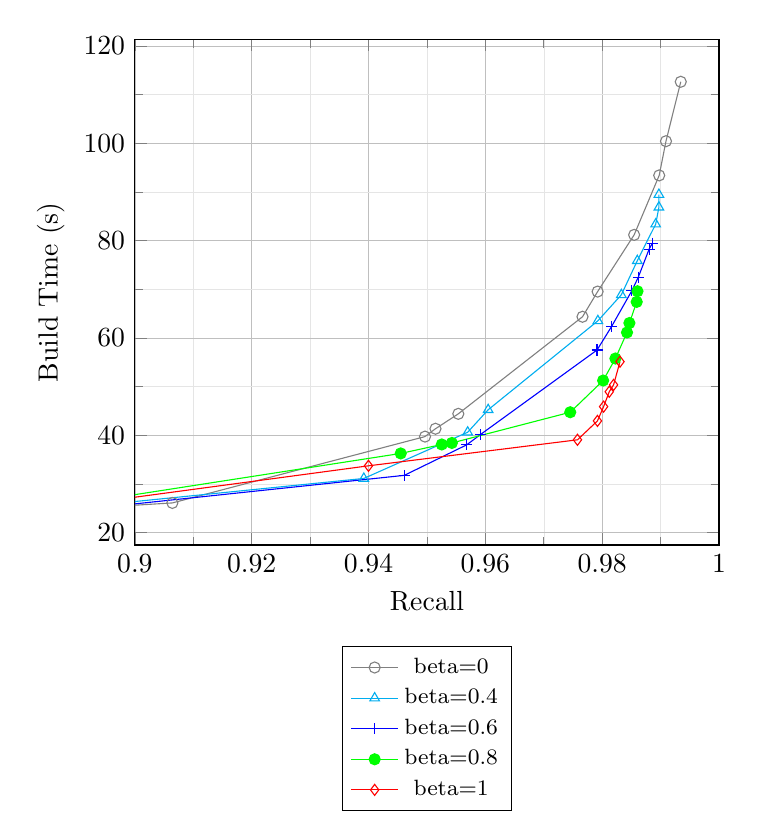
\begin{tikzpicture}
        \begin{axis}[
            xlabel={ Recall },
            ylabel={ Build Time (s) },
            xmin=0.9,
            xmax=1,  % 设置x轴范围
            yticklabel style={/pgf/number format/fixed,
                              /pgf/number format/precision=2},
            legend style={font=\footnotesize, at={(0.5,-0.2)}, anchor=north},
            grid=both,
            major grid style={line width=.2pt,draw=gray!50}, 
            minor grid style={line width=.1pt,draw=gray!20}, 
            width=9cm, % 设置图宽度
    height=8cm, % 设置图高度
            mark size=2pt,
            minor tick num=1
        ]

        \addplot[mark=o, color=gray] coordinates {
    (0.63849, 6.44658)
    (0.90642, 26.0727)
    (0.94967, 39.7029)
    (0.95146, 41.3137)
    (0.95537, 44.3801)
    (0.97663, 64.3235)
    (0.97922, 69.4988)
    (0.98547, 81.1507)
    (0.98976, 93.3715)
    (0.99092, 100.402)
    (0.99345, 112.61)
};
\addlegendentry{beta=0};

% \addplot[mark=diamond*, color=blue] coordinates {
%     (0.67171, 9.27315)
%     (0.91537, 28.2885)
%     (0.95399, 42.4314)
%     (0.95883, 48.6772)
%     (0.95321, 34.8281)
%     (0.97901, 69.4469)
%     (0.98367, 78.7338)
%     (0.97663, 65.0007)
%     (0.98562, 80.9125)
%     (0.98983, 91.8779)
%     (0.9906, 98.2263)
%     (0.99247, 102.164)
% };
% \addlegendentry{beta=0.1};

% \addplot[mark=square, color=magenta] coordinates {
%     (0.72903, 11.29)
%     (0.92474, 28.8489)
%     (0.95315, 35.3782)
%     (0.95382, 41.5403)
%     (0.95665, 47.0555)
%     (0.97722, 63.1549)
%     (0.97884, 66.1246)
%     (0.98239, 74.181)
%     (0.98532, 78.3121)
%     (0.98876, 87.1786)
%     (0.99035, 91.1609)
%     (0.99099, 95.2748)
% };
% \addlegendentry{beta=0.2};

% \addplot[mark=diamond*, color=blue] coordinates {
%     (0.79548, 14.5856)
%     (0.93635, 30.7995)
%     (0.95523, 41.7689)
%     (0.96188, 46.646)
%     (0.96207, 37.531)
%     (0.97893, 65.5793)
%     (0.98429, 71.5846)
%     (0.98174, 64.1363)
%     (0.98533, 77.4092)
%     (0.98993, 85.9305)
%     (0.99027, 90.0223)
%     (0.99136, 93.0512)
% };
% \addlegendentry{beta=0.3};

\addplot[mark=triangle, color=cyan] coordinates {
    (0.81585, 16.1813)
    (0.93919, 31.101)
    (0.95697, 40.5958)
    (0.96048, 45.2127)
    (0.97926, 63.4894)
    (0.98328, 68.8376)
    (0.98601, 75.8341)
    (0.98916, 83.3571)
    (0.98971, 86.8256)
    (0.98971, 89.4334)
};
\addlegendentry{beta=0.4};

% \addplot[mark=square*, color=blue] coordinates {
%     (0.83046, 17.6968)
%     (0.94216, 31.5284)
%     (0.95587, 39.4981)
%     (0.95906, 43.5703)
%     (0.96702, 38.2888)
%     (0.97759, 60.4692)
%     (0.9818, 65.4958)
%     (0.98182, 61.7801)
%     (0.98545, 73.6448)
%     (0.98852, 79.5831)
%     (0.98814, 83.0528)
%     (0.98945, 84.5389)
% };
% \addlegendentry{beta=0.5};

\addplot[mark=+, color=blue] coordinates {
    (0.84976, 19.4923)
    (0.94612, 31.7386)
    (0.95681, 38.0106)
    (0.95914, 40.1051)
    (0.97912, 57.4923)
    (0.98161, 62.3296)
    (0.98508, 69.68)
    (0.98618, 72.4512)
    (0.98804, 78.2353)
    (0.9886, 79.4475)
};
\addlegendentry{beta=0.6};

% \addplot[mark=square*, color=blue] coordinates {
%     (0.86574, 20.3125)
%     (0.94814, 31.0685)
%     (0.95757, 36.9108)
%     (0.95926, 39.9212)
%     (0.97403, 38.1749)
%     (0.97948, 53.6777)
%     (0.98136, 59.3345)
%     (0.98456, 58.0657)
%     (0.98619, 66.2935)
%     (0.98557, 70.4287)
%     (0.98746, 73.314)
%     (0.98776, 75.3228)
% };
% \addlegendentry{beta=0.7};

\addplot[mark=*, color=green] coordinates {
    (0.86774, 21.77)
    (0.94551, 36.2417)
    (0.95254, 38.0826)
    (0.95427, 38.3943)
    (0.97453, 44.7067)
    (0.98016, 51.2206)
    (0.98226, 55.7463)
    (0.98425, 61.1023)
    (0.98466, 63.0378)
    (0.98591, 67.3815)
    (0.98604, 69.5683)
};
\addlegendentry{beta=0.8};

% \addplot[mark=x, color=blue] coordinates {
%     (0.8693, 23.4329)
%     (0.94482, 31.432)
%     (0.95088, 34.8743)
%     (0.95159, 36.7078)
%     (0.97548, 38.3315)
%     (0.9772, 48.2002)
%     (0.97943, 52.0249)
%     (0.98322, 53.7999)
%     (0.9844, 57.7625)
%     (0.98509, 59.6632)
%     (0.98615, 62.5879)
%     (0.98551, 63.7582)
% };
% \addlegendentry{beta=0.9};

\addplot[mark=diamond, color=red] coordinates {
    (0.8835, 24.5845)
    (0.93999, 33.6991)
    (0.97577, 39.0443)
    (0.97919, 42.9276)
    (0.98024, 45.8562)
    (0.98121, 48.9165)
    (0.98195, 50.3317)
    (0.98305, 55.1036)
};
\addlegendentry{beta=1};

    \end{axis}
\end{tikzpicture}
\caption{Recall vs Build Time, based on different beta values. Down and to the right is better.(在重新跑代码,会有改动,数据还未更新)}
\label{fig4}
\end{figure}

% \begin{figure}
%     \centering
%     \begin{tikzpicture}
%         \begin{axis}[
%             xlabel={ Recall },
%             ylabel={ Build Time (s) },
%             xmin=0.85, xmax=0.98,  % 设置x轴范围
%             ymin=5, ymax=50,  % 设置y轴范围
%             yticklabel style={/pgf/number format/fixed,
%                               /pgf/number format/precision=2},
%             legend style={font=\footnotesize, at={(0.5,-0.2)}, anchor=north},
%             grid=both,
%             major grid style={line width=.2pt,draw=gray!50}, 
%             minor grid style={line width=.1pt,draw=gray!20}, 
%             minor tick num=1
%         ]
%             % 绘制数据点
%             \addplot[mark=o, color=blue] coordinates {
%                 (0.85216, 7.14549)
%                 (0.88053, 10.5071)
%                 (0.90786, 14.7031)
%                 (0.92565, 18.589)
%                 (0.94244, 22.6255)
%                 (0.95325, 26.5892)
%                 (0.95926, 30.1845)
%                 (0.96601, 33.8144)
%                 (0.9697, 36.8853)
%                 (0.9734, 39.6411)
%                 (0.97596, 42.0721)
%                 (0.97748, 44.2723)
%                 (0.97771, 45.8237)
%                 (0.97825, 46.9734)
%                 (0.97847, 48.3685)
%             };
%             \addlegendentry{beta=0};
            
%             \addplot[mark=triangle*, color=red] coordinates {
%                 (0.86016, 9.5658)
%                 (0.88587, 13.1555)
%                 (0.91509, 17.123)
%                 (0.93322, 20.9797)
%                 (0.9462, 24.9616)
%                 (0.95688, 29.0038)
%                 (0.96432, 32.5156)
%                 (0.96848, 35.6272)
%                 (0.9704, 38.4648)
%                 (0.9721, 40.8545)
%                 (0.97422, 42.0836)
%                 (0.9754, 43.3568)
%                 (0.97558, 45.0875)
%                 (0.97652, 46.1845)
%                 (0.97668, 47.2488)
%             };
%             \addlegendentry{beta=0.1}

%             \addplot[mark=square*, color=green] coordinates {
%                 (0.86141, 11.4528)
%                 (0.90234, 14.8085)
%                 (0.92336, 18.4268)
%                 (0.94095, 21.8741)
%                 (0.94821, 25.4952)
%                 (0.9596, 29.019)
%                 (0.96419, 32.1485)
%                 (0.97034, 34.7239)
%                 (0.97174, 37.2602)
%                 (0.97289, 39.4556)
%                 (0.97512, 41.132)
%                 (0.97687, 42.9331)
%                 (0.97723, 44.3959)
%                 (0.97756, 45.0601)
%                 (0.97786, 45.7309)
%             };
%             \addlegendentry{beta=0.2};

%             \addplot[mark=diamond*, color=red] coordinates {
%                 (0.87519, 14.7437)
%                 (0.91766, 18.1554)
%                 (0.93637, 21.6574)
%                 (0.94888, 24.8686)
%                 (0.95668, 28.1587)
%                 (0.9632, 31.3316)
%                 (0.96803, 34.079)
%                 (0.97098, 38.9735)
%                 (0.97157, 39.0298)
%                 (0.97375, 43.3107)
%                 (0.9744, 42.3344)
%                 (0.9755, 43.6316)
%                 (0.97605, 44.6157)
%                 (0.97676, 45.3245)
%                 (0.9767, 46.8015)
%             };
%             \addlegendentry{beta=0.3};

%             \addplot[mark=*, color=blue] coordinates {
%                 (0.87727, 16.5579)
%                 (0.92463, 20.0414)
%                 (0.93639, 23.1683)
%                 (0.94932, 26.1813)
%                 (0.95873, 28.9158)
%                 (0.96302, 31.4993)
%                 (0.96814, 34.2085)
%                 (0.97038, 36.5745)
%                 (0.97222, 38.3839)
%                 (0.97295, 40.2648)
%                 (0.97482, 41.6111)
%                 (0.97516, 42.489)
%                 (0.9756, 43.8622)
%                 (0.97525, 44.5176)
%                 (0.97592, 45.1228)
%             };
%             \addlegendentry{beta=0.4};

%             \addplot[mark=o, color=green] coordinates {
%                 (0.87854, 18.7242)
%                 (0.92624, 21.5712)
%                 (0.94179, 24.3059)
%                 (0.95096, 27.4755)
%                 (0.95829, 30.4188)
%                 (0.96306, 32.7788)
%                 (0.96639, 34.7165)
%                 (0.96948, 37.4017)
%                 (0.97155, 38.8314)
%                 (0.97335, 39.6699)
%                 (0.974, 40.6206)
%                 (0.97471, 41.8275)
%                 (0.97506, 42.395)
%                 (0.97522, 42.9642)
%                 (0.97487, 43.4961)
%             };
%             \addlegendentry{beta=0.5};

%             \addplot[mark=o, color=purple] coordinates {
%                 (0.88194, 21.009)
%                 (0.93323, 24.1251)
%                 (0.94658, 26.8905)
%                 (0.95661, 29.2486)
%                 (0.9612, 31.5305)
%                 (0.96556, 33.6264)
%                 (0.96868, 35.5556)
%                 (0.9684, 36.9178)
%                 (0.971, 38.5146)
%                 (0.97076, 39.8063)
%                 (0.97199, 40.6961)
%                 (0.97219, 41.7333)
%                 (0.97289, 42.5281)
%                 (0.97363, 42.8981)
%                 (0.9731, 43.7076)
%             };
%             \addlegendentry{beta=0.6};

%             \addplot[mark=o, color=brown] coordinates {
%                 (0.8831, 21.958)
%                 (0.94042, 24.8997)
%                 (0.95201, 27.2785)
%                 (0.95694, 30.1228)
%                 (0.95954, 31.8615)
%                 (0.9639, 33.5073)
%                 (0.96686, 35.473)
%                 (0.96756, 36.3597)
%                 (0.96812, 37.5114)
%                 (0.97012, 38.6334)
%                 (0.97126, 39.5456)
%                 (0.97077, 40.2533)
%                 (0.9714, 40.6524)
%                 (0.97166, 41.5013)
%                 (0.97166, 42.0031)
%             };
%             \addlegendentry{beta=0.7};

%             \addplot[mark=o, color=purple] coordinates {
%                 (0.88046, 25.3031)
%                 (0.93618, 26.2645)
%                 (0.94859, 29.3404)
%                 (0.95418, 31.0457)
%                 (0.95676, 32.9544)
%                 (0.96034, 31.2504)
%                 (0.96174, 32.4726)
%                 (0.96372, 33.7332)
%                 (0.9645, 34.7429)
%                 (0.96484, 35.5458)
%                 (0.96576, 35.997)
%                 (0.96605, 36.3571)
%                 (0.96639, 36.7068)
%                 (0.96712, 37.2443)
%                 (0.96679, 37.5571)
%             };
%             \addlegendentry{beta=0.8};

%             \addplot[mark=o, color=orange] coordinates {
%                 (0.88197, 23.8484)
%                 (0.93602, 26.4575)
%                 (0.94984, 28.2043)
%                 (0.95562, 29.7106)
%                 (0.95819, 30.871)
%                 (0.96046, 31.7734)
%                 (0.96024, 32.5655)
%                 (0.96164, 33.0505)
%                 (0.96321, 33.622)
%                 (0.96319, 34.3168)
%                 (0.96256, 34.8853)
%                 (0.96278, 35.1636)
%                 (0.96316, 35.6895)
%                 (0.96301, 35.9322)
%                 (0.96308, 36.2538)
%             };
%             \addlegendentry{beta=0.9};

%         \addplot[mark=square*, color=blue] coordinates {
%                 (0.88046, 24.4364)
%                 (0.93773, 26.6966)
%                 (0.94697, 28.0993)
%                 (0.95175, 29.1162)
%                 (0.95314, 29.8875)
%                 (0.95488, 30.2619)
%                 (0.95534, 30.691)
%                 (0.95559, 30.9319)
%                 (0.95516, 31.4961)
%                 (0.95542, 31.603)
%                 (0.95506, 31.8962)
%                 (0.95512, 32.1614)
%                 (0.9551, 32.6388)
%                 (0.9552, 32.709)
%                 (0.9552, 33.0651)
%             };
%             \addlegendentry{beta=1};

%         \end{axis}
%     \end{tikzpicture}
%     \caption{Recall vs Build Time, based on different beta values. Down and to the right is better.}
%     \label{}
% \end{figure}

\newpage

\bgroup\small
\bibliographystyle{ieeetr}
\let\xxx=\bibitem\def\bibitem{\par\vspace{1mm}\xxx}
\bibliography{add}
\egroup

\end{document}
